%! TeX program = lualatex
\documentclass[article]{luvita}

\title{Luvita Hieroglífico: Panorama geral da língua e contexto histórico}
\author{Caio Geraldes}
\date{19 de maio de 2025}

\addbibresource{../../../Bibliografia/biblio.bib}



\begin{document}

\frontmatter

\mainmatter%

\maketitle

\chapter{Descobrimento e decifração}

\section{Primeiras descobertas}

\begin{compactitem}
	\item Documentos começam a ser encontrados no século XIX no norte da Síria,
	Anatólia e Iraque (\autoref{fig:mapa19}).
	\begin{compactitem}
		\item ``Pedras hamatitas'' (\autoref{fig:hama2}) são os primeiros documentos e
		foram vistas por~\citet[146--7]{Burckhardt1822} em um bazar em Hamath em
		1812 e apenas publicadas em ``traçados'' -- bastante rudimentares --
		em~\citet[333--60]{UnexploredSyriaI}.
		\item Antes da publicação de Burton e Drake, outras inscrições monumentais
		com hieróglifos são encontradas\slash{}vistas e identificadas como
		pertencendo ao mesmo sistema de escrita das ``pedras hamatitas'' em
		Yazılıkaya e Nişantaş (próximas de Boğazköy-Hattusa) e İvriz (Cilicia
		Aspera) na Anatólia central, em Sipylos (Akpınar) e Karabel na Anatólia
		ocidental e Aleppo na Síria (\autoref{fig:yazilikaya} e~\autoref{fig:aleppo}).
		\item Também são encontrados selos\slash{}\emph{bullae} em Nineveh no
		Iraque (\autoref{fig:nineveh}) e o selo digráfico conhecido como
		``Tarkondemos'', talvez de İzmir, (\autoref{fig:tarkondemos}).
	\end{compactitem}
	\item Em 1876, Sayce propõe, em uma palestra para a Society of Biblical
	Archaeology,\footnote{Transcrita no \emph{Transactions of the Society of
			Biblical Archaeology} v. V, pp.22--32, disponível no
		\hrf{https://archive.org/details/transactionssoc04nashgoog}{Internet
			Archive}.} associar a língua dos hieróglifos ao povo conhecido pelo Antigo
	Testamento como \emph{Hititas} e pelos textos então recém decifrados em
	egípcio e neo-assírio com o povo do país de \emph{Hatti}.
\end{compactitem}

\begin{figure}[htb]
	\begin{center}
		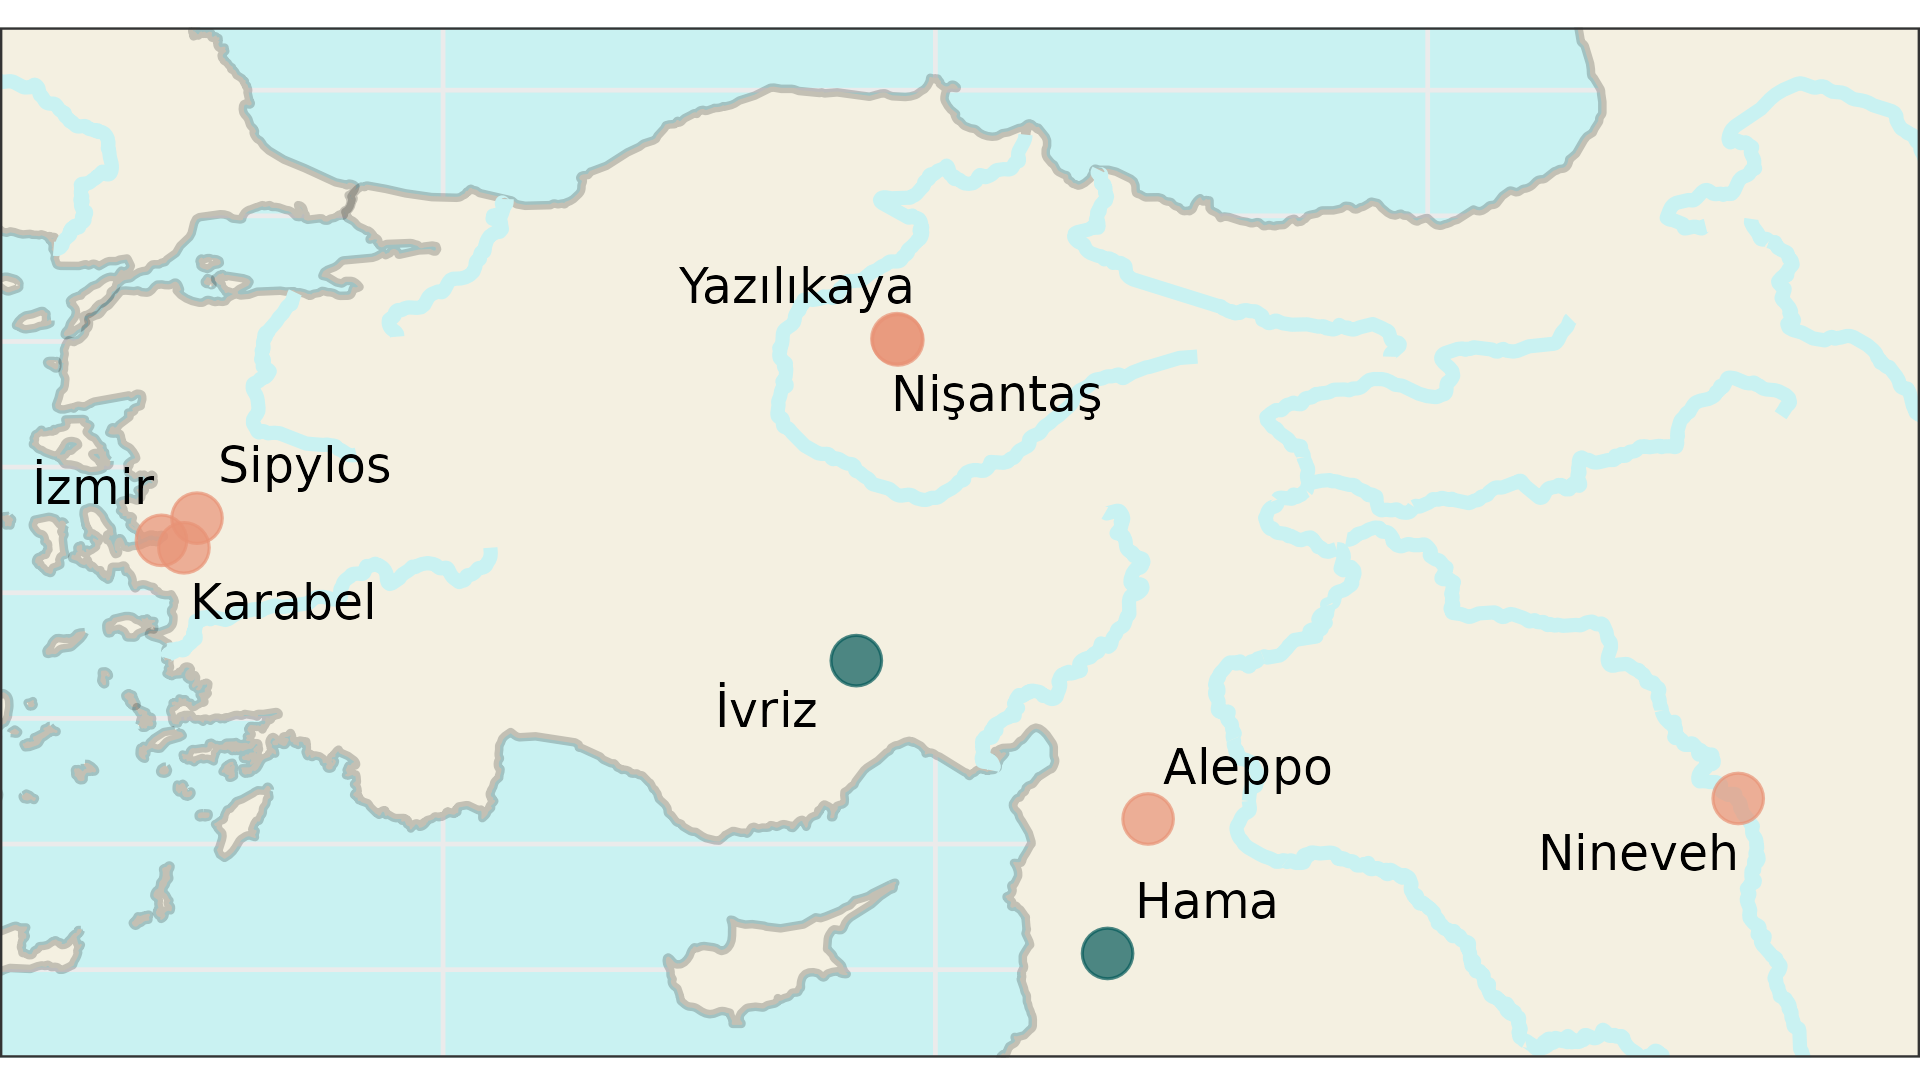
\includegraphics[width=\textwidth]{../../../Mídia/Map19.png}
	\end{center}
	\caption{Mapa das inscrições identificadas no século XIX\@. Pontos laranjas
		denotam inscrições do período Imperial e pontos verdes as do período
		Neo-Hitita.}\label{fig:mapa19}
\end{figure}

\begin{figure}[htb]
	\centering
	\begin{subfigure}{0.49\textwidth}
		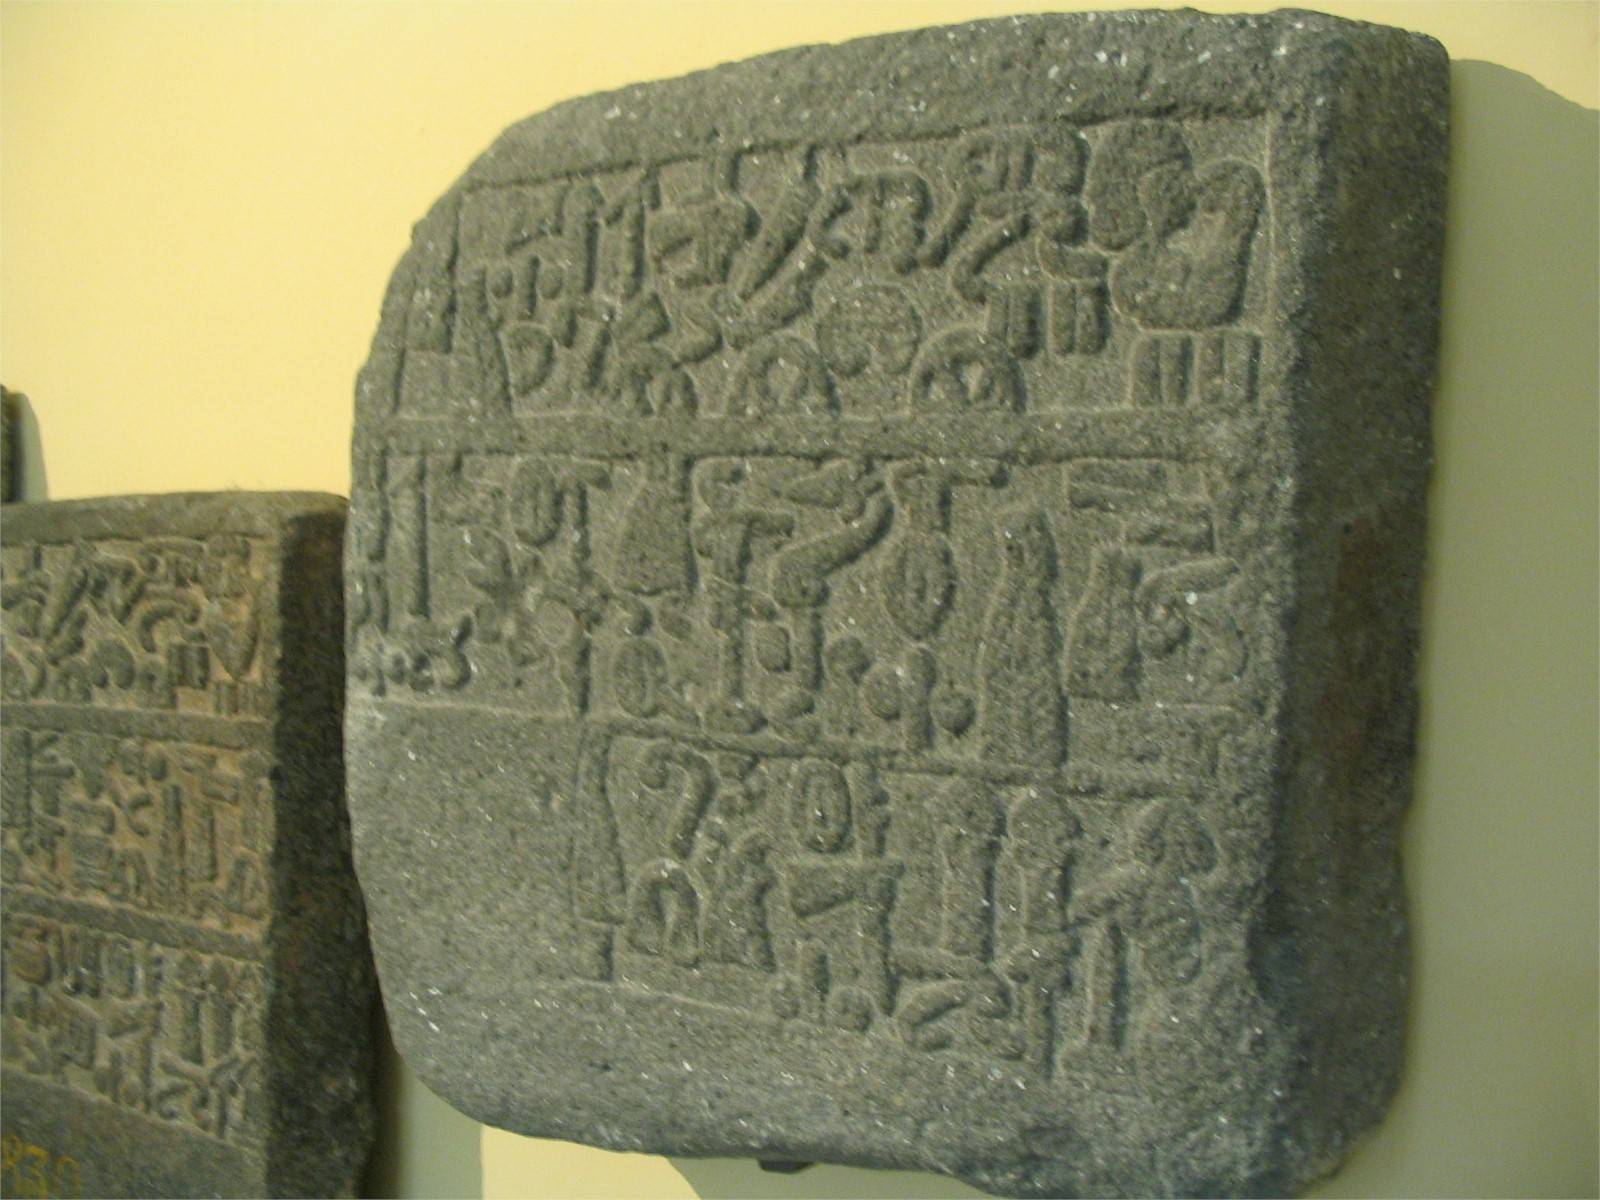
\includegraphics[width=\textwidth]{../../../Mídia/hama08.jpg}
	\end{subfigure}
	\begin{subfigure}{0.49\textwidth}
		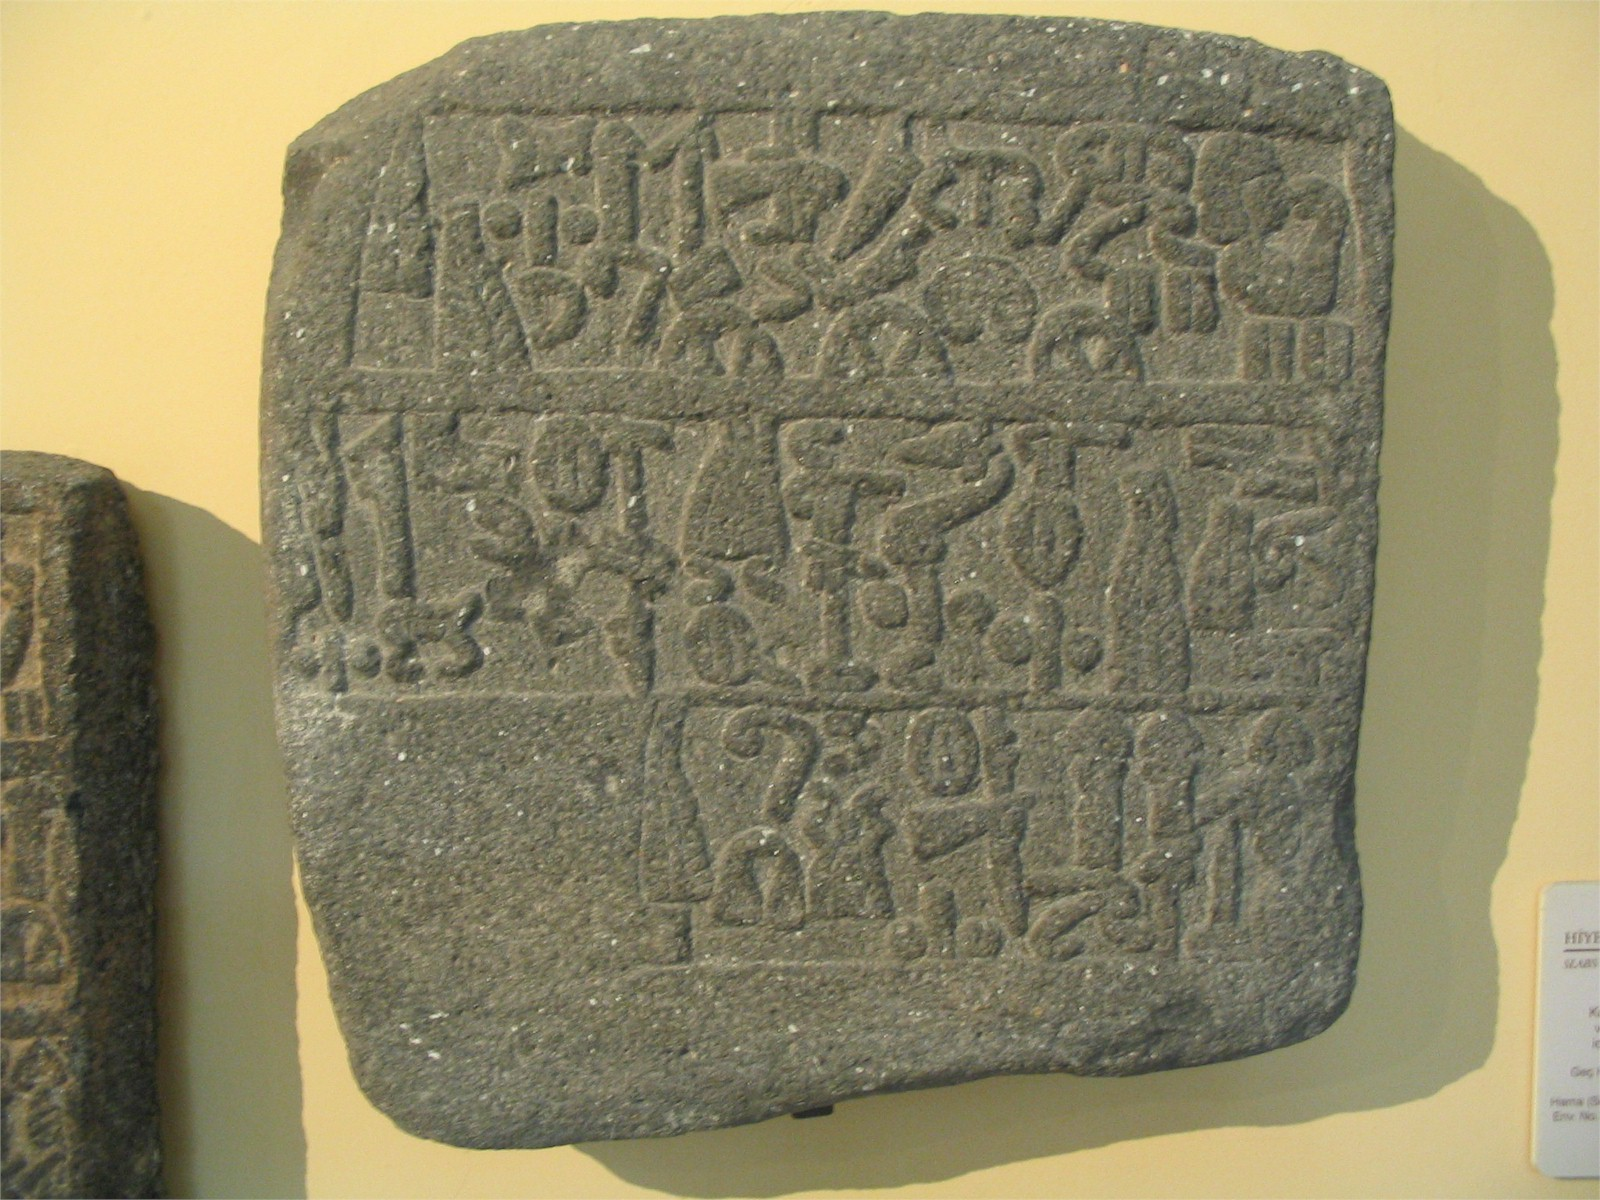
\includegraphics[width=\textwidth]{../../../Mídia/hama09.jpg}
	\end{subfigure}
	\caption[HAMA 2]{Inscrição HAMA 2. Dimensões da inscrição:
		0.36\times0.31m.
		Imagens de Bora Bilgin, 2006,
		disponíveis em
		\href{https://www.hittitemonuments.com/hama/}{Hittite Monuments}.
		Edição e traçado em~\citeabbrev*{CHLI11}, pp.\ 411ff.\ e \emph{plates}
		221--2.
	}\label{fig:hama2}
\end{figure}

\begin{figure}[htb]
	\begin{center}
		\includegraphics[width=\textwidth]{../../../Mídia/yazilikaya.png}
	\end{center}
	\caption{YAZILIKAYA, no. 81 (Câmara A).
		Relevo de Tudhaliya IV com seu nome em hieróglifos, 𔐒𔐃𔐒 MAGNUS+REX
		MONS\textsubscript{2} MAGNUS+REX\@.
		Imagens de Cüneyt Süer, 2011,
		disponíveis em
		\href{https://www.hittitemonuments.com/hama/}{Hittite Monuments}.
	}\label{fig:yazilikaya}
\end{figure}

\begin{figure}[htb]
	\begin{center}
		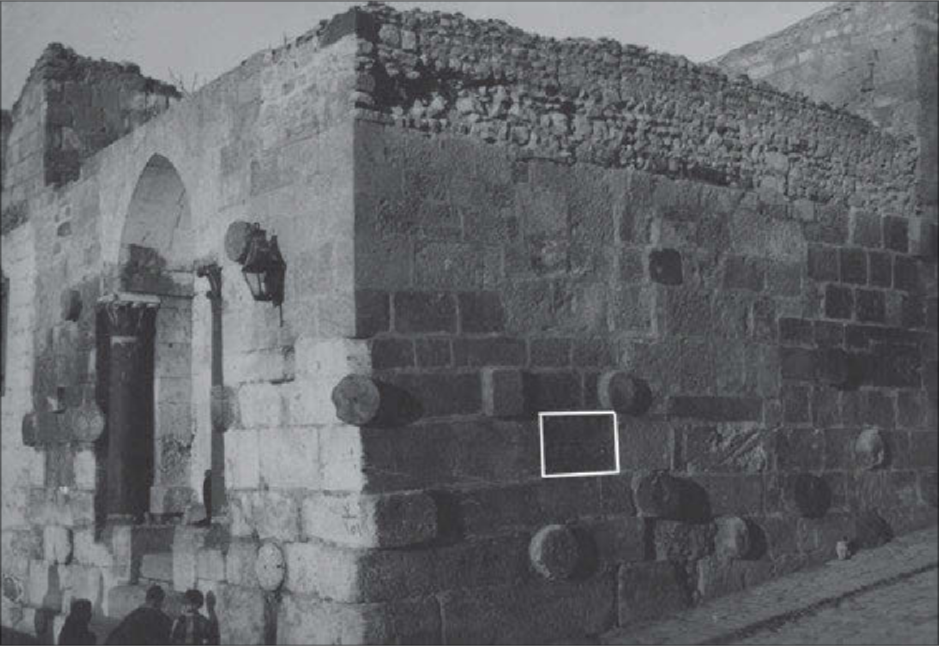
\includegraphics[width=\textwidth]{../../../Mídia/aleppo1a.png}
		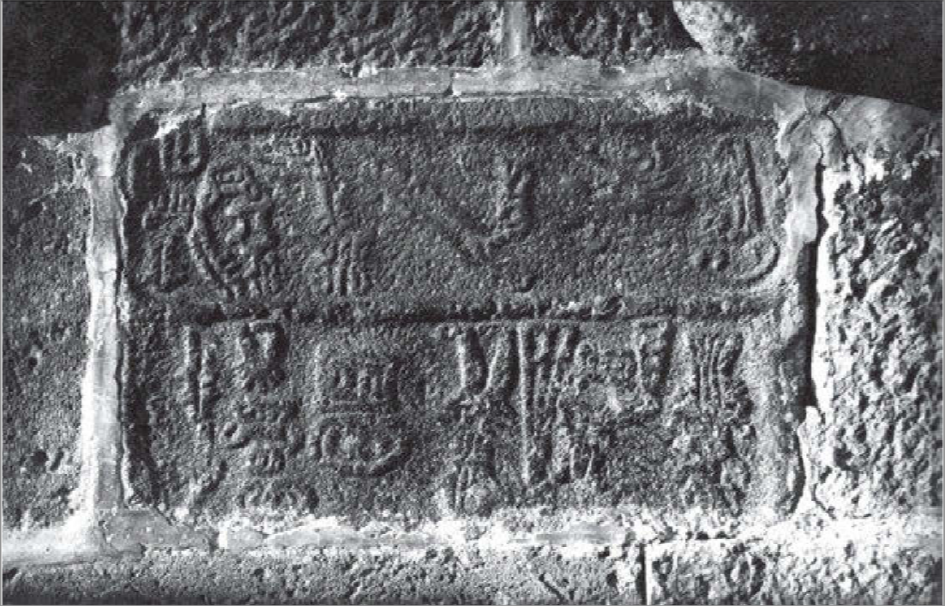
\includegraphics[width=\textwidth]{../../../Mídia/aleppo1b.png}
	\end{center}
	\caption{Inscrição ALEPPO 1 em seu contexto de descoberta (como relatado
		por~\citet{UnexploredSyriaI}), fotos de. Atualmente no museu de Ankara.
		Edição e traçado em~\citeabbrev*{CHLI3}, pp.\ 14ff.\ e \emph{plates} 4--5.}\label{fig:aleppo}
\end{figure}

\begin{figure}[htb]
	\begin{center}
		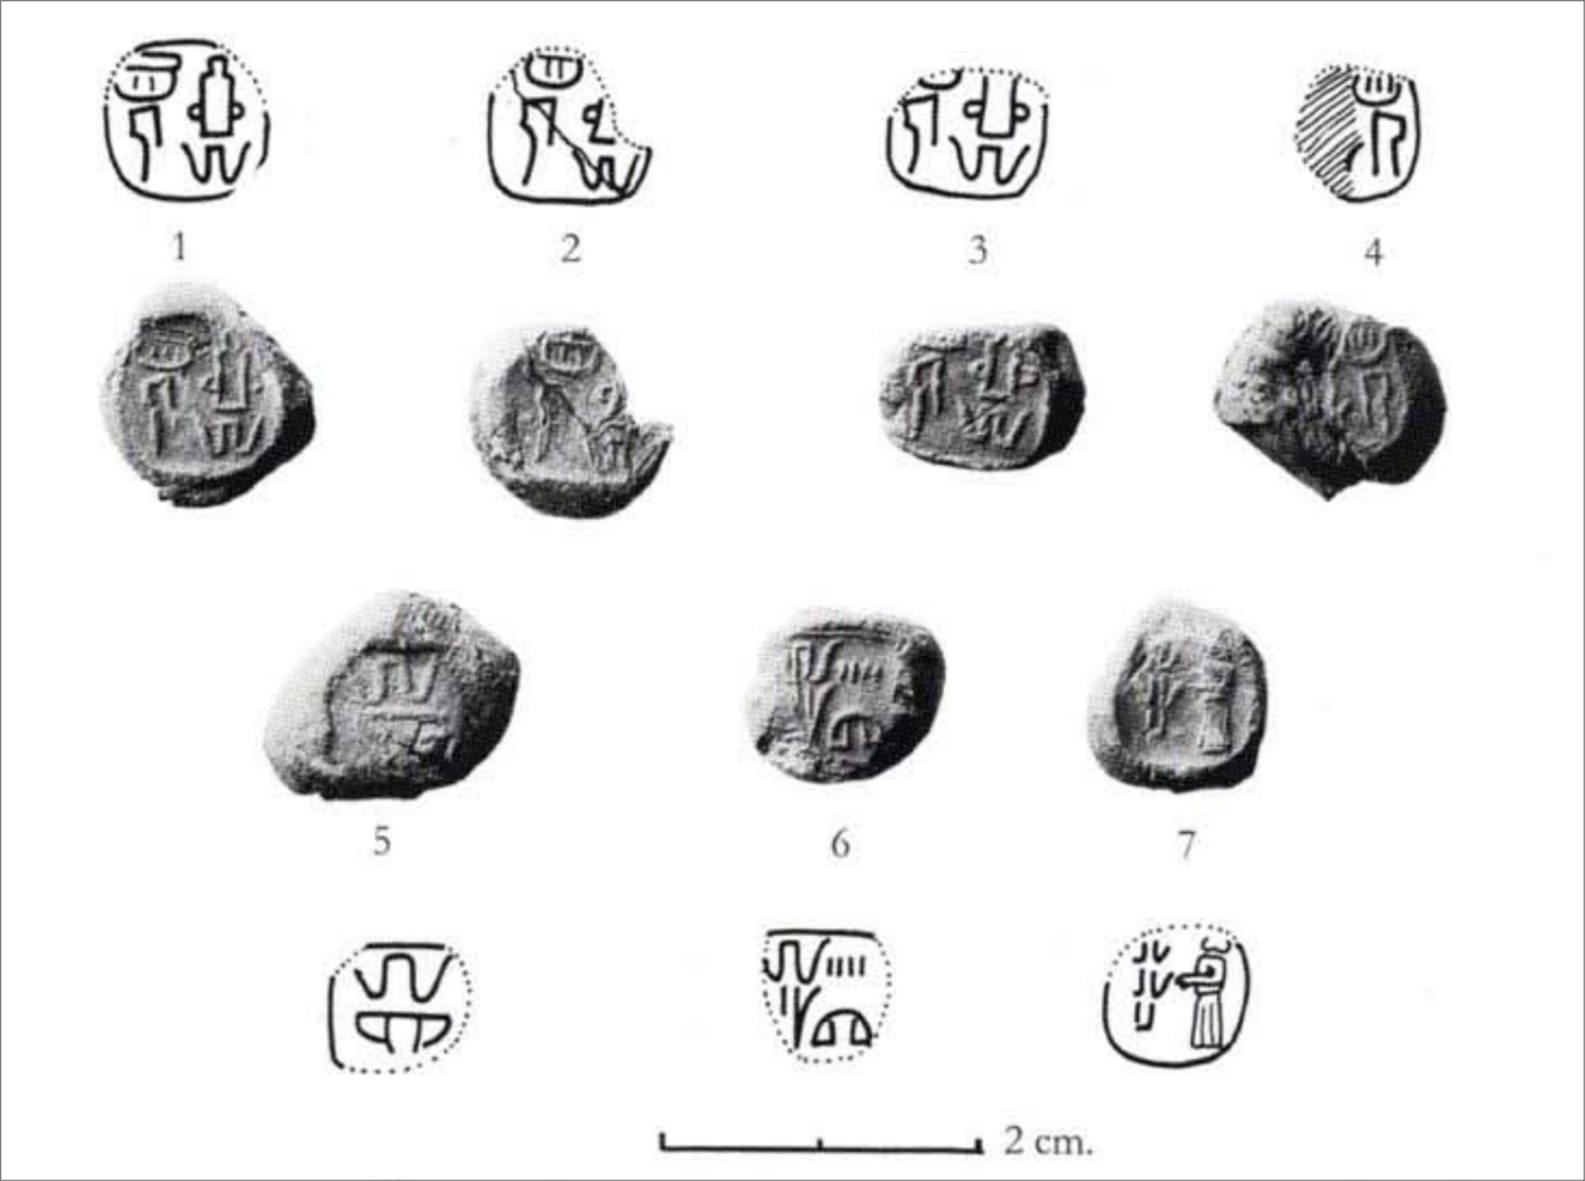
\includegraphics[width=\textwidth]{../../../Mídia/nineveh.png}
	\end{center}
	\caption{\emph{Bullae} de Nineveh 1--7. Aprox. 10mm\times10mm. Imagens
		de~\citeabbrev*{CHLI13}, \emph{plate} 332. Edição e traçado
		em~\citeabbrev*{CHLI11}.}\label{fig:nineveh}
\end{figure}

\begin{figure}[htb]
	\begin{center}
		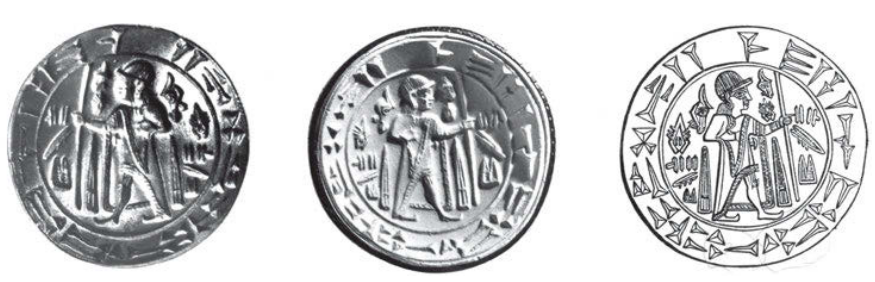
\includegraphics[width=\textwidth]{../../../Mídia/tarkondemos.png}
	\end{center}
	\caption{Selo de ``Tarkondemos''. Digráfico com cuneiforme na circunferência e
		hieróglifos no centro. Atualmente o texto é interpretado como pertencente a
		um certo \emph{Tarkas{(sa)}nawa}. Final do século \textsc{xii aec}.
		Atualmente em Walters Art Gallery, Baltimore, no. 57.1512.
		Imagem e traçado de~\citet[p. 45f.; \emph{plate} 32]{CHLI3}
	}\label{fig:tarkondemos}
\end{figure}

\clearpage
\section{Os outros hititas}

\begin{compactitem}
	\item Em 1906, ocorre a escavação de Hattusa em Boğazköy/Boğazkale e de seus
	documentos em cuneiforme.
	\item Entre 1915--17, Bedřich Hrozný demonstra que a língua do cuneiforme de
	Boğazköy é indo-europeia e propõe um primeiro esboço gramatical.
	\item A língua dos textos cuneiformes de Hattusa passa a ser entendida como a
	língua dos hititas e começa-se a interpretar os textos
	\item Dentro dos textos em hitita, há passagens que o escriba avisa que devem
	ser lidas \emph{luwili}, isto é, ``em luvita''.
	\item Algumas palavras ao longo dos textos são precedidas de sinal cuneiforme,
	\foreignlanguage{hittite}{𒃵}, chamado pelo nome alemão \emph{Glossenkeil},
	isto é, ``cunha de glosa/palavra estrangeira''. Os termos precedidos de
	\emph{Glossenkeil}s são atribuídos a uma língua hipotética
	\emph{Glossenkeilsprache}.
	\item Ao longo da primeira metade do século XX, tenta-se ler nos hieróglifos
	anatólicos o hitita, mas de maneira insatisfatória.
	\item Entre 1940 e 1960 são publicados partes da inscrição bilíngue de
	Karatepe-Aslantaş (Cilícia) em fenício e hieróglifos anatólicos, descoberta
	pelo professore de ensino fundamental Ekrem Kuşçu em 1927 e escavada por Bossert e
	Halet Çambel a partir de 1946 (\autoref{fig:portaoU} e
	\autoref{fig:karatepe_a}).
	\item Em 1974, são publicadas as ``Novas leituras'' de quatro hieróglifos
	por~\textcite{HawkinsMorpurgoNeumann1974}, pelas quais se permite identificar
	língua dos hieróglifos hititas com a
	\emph{\foreignlanguage{german}{Glossenkeilsprache}} e dos cuneiformes que deveriam
	ser lidos \emph{luwili}.
	\item Daí em diante, estas línguas passaram a ser conhecidas respectivamente como
	\emph{luvita hieroglífico} e \emph{luvita cuneiforme}.
\end{compactitem}


\begin{figure}[b]
	\begin{center}
		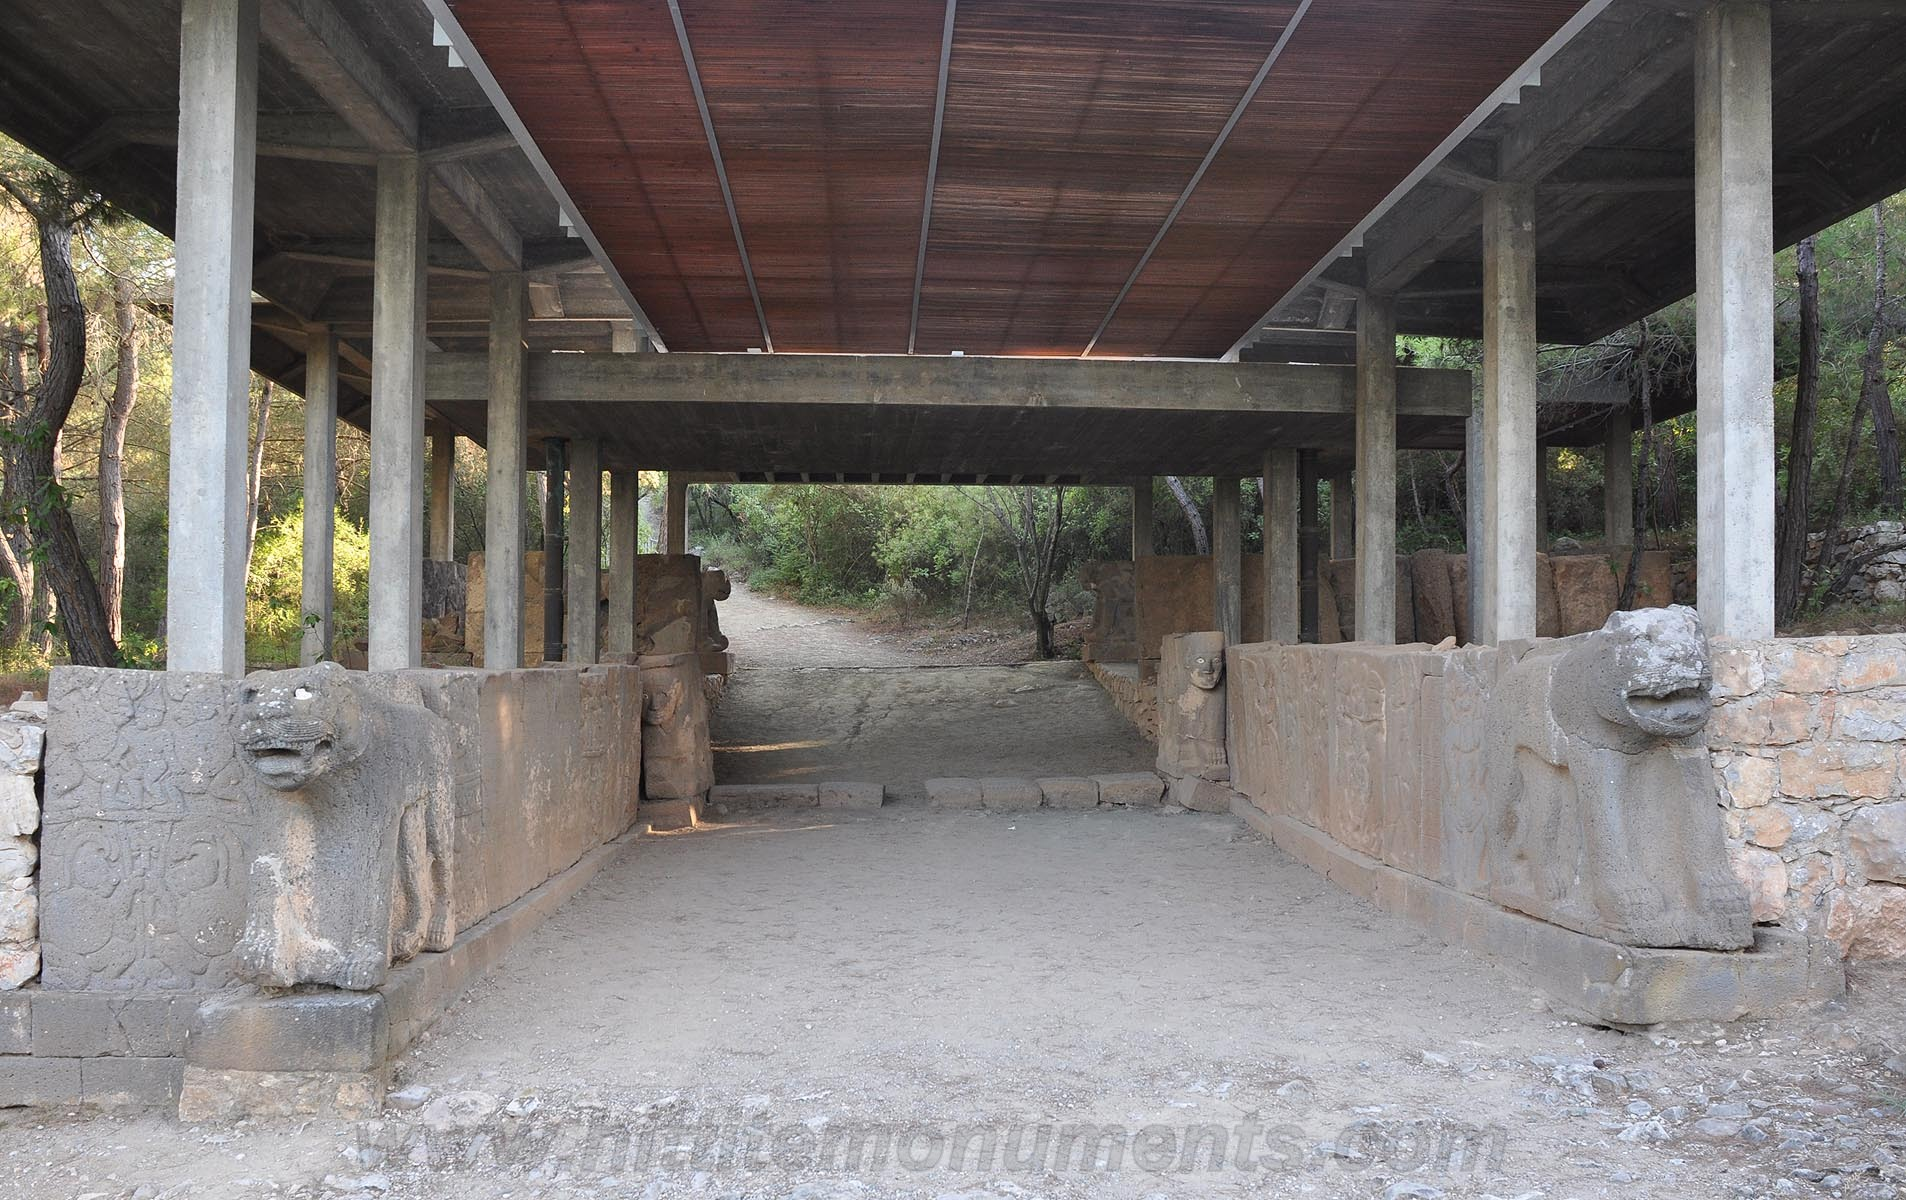
\includegraphics[width=0.80\textwidth]{../../../Mídia/karatepe01.jpg}
	\end{center}
	\caption[Portão Inferior (Norte) de Karatepe]{Portão Inferior (Norte) de
		Karatepe.
		Imagem de Bora Bilgin, 2008, disponível em
		\href{https://www.hittitemonuments.com/karatepe}{Hittite Monuments}.
	}\label{fig:portaoU}
\end{figure}
\begin{figure}
	\begin{center}
		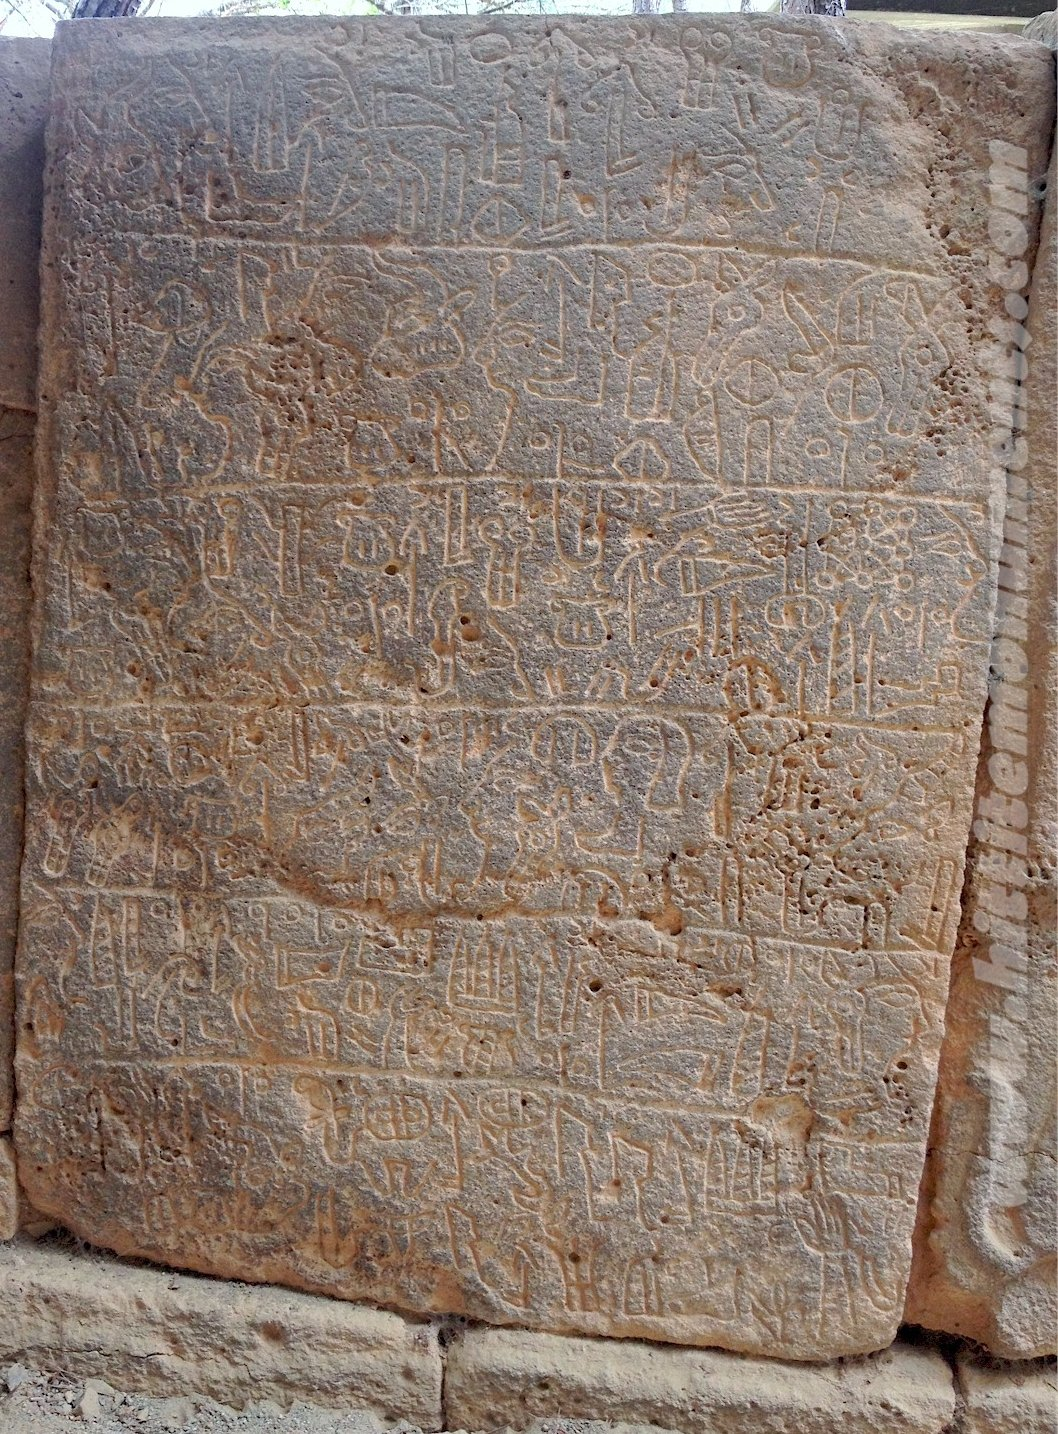
\includegraphics[width=0.85\textwidth]{../../../Mídia/karatepe58.jpg}
		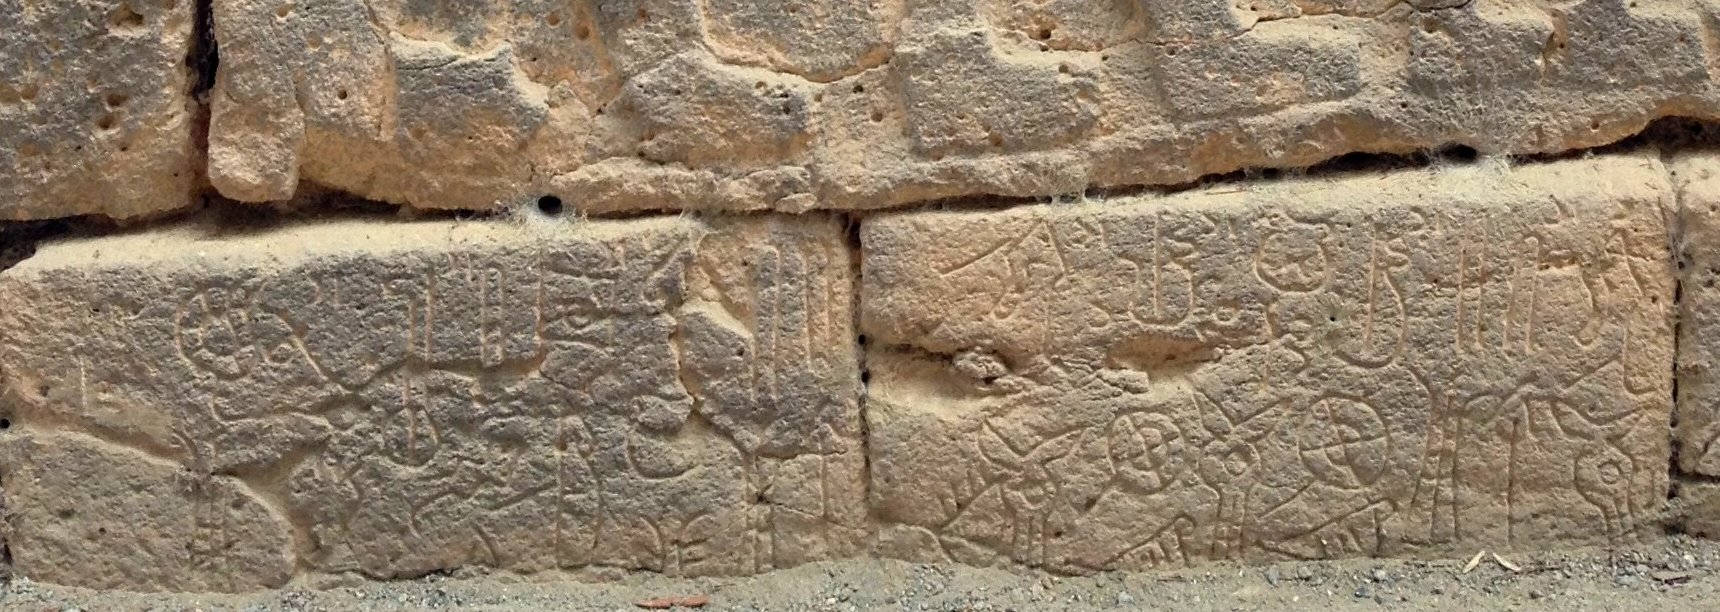
\includegraphics[width=0.85\textwidth]{../../../Mídia/karatepe104.jpg}
	\end{center}
	\caption[Ortostatos de Karatepe (Portão Inferior)]{Ortostatos de Karatepe
		(Portão Inferior).
		Imagens de Bora Bilgin, 2008, disponível em
		\href{https://www.hittitemonuments.com/karatepe}{Hittite Monuments}.
	}\label{fig:karatepe_a}
\end{figure}

\chapter{Datação e geografia}

\noindent Datação:

\begin{compactitem}
	\item Os textos em luvita cuneiforme se encontram junto de textos hititas
	datados dos séculos \textsc{xvi} e \textsc{xv} \textsc{aec}.\footnote{Datação de
		\citet{Starke1985}.}
	\item Os textos em luvita hieroglífico se dividem entre:
	\begin{compactitem}
		\item Imperiais: contemporâneos ao império hitita, entre os reinados de
		Arnuwanda I (apenas selos) e Tudhaliya IV ou Suppiluliuma II (inscrições
		monumentais), \emph{circa} 1400--1300 \textsc{aec}.
		\item Neo-hititas: produzidos nas cidades-estado posteriores à dissolução do
		império hitita que entraram na esfera de influência dos Assírios entre 1100
		e 700 \textsc{aec}.
	\end{compactitem}
\end{compactitem}


\noindent Regiões da idade do bronze\slash{}período imperial:
\begin{compactitem}
	\item Lúvia / Arzawa:
	\begin{compactitem}
		\item um território chamado Lúvia é conhecido das leis hititas do segundo
		milênio.\footnote{\emph{Luwiya}, hit.\ \mbox{\textsc{kur}}
			\mbox{\textit{Lu-ú-i-ya}}. CTH 291 e 292. Tradução das leis em
			\textcite{Hoffner1997}.}
		\item o território também é chamado por Arzawa.
		\item corresponde à Anatólia ocidental.
	\end{compactitem}
	\item Wilusa e Ahhiyawa:
	\begin{compactitem}
		\item por vezes tratada separadamente da Lúvia / Arzawa.
		\item zona de contato com micênicos.
		\item a palavra hitita \emph{Wilusa} provavelmente é cognata do grego Ἴλιον
		(Ílion).
		\item costa da Anatólia ocidental
	\end{compactitem}
	\item Kizzuwatna
	\begin{compactitem}
		\item poucos documentos em hitita hieroglífico.
		\item conhecida sobretudo pelos textos de culto hitita em luvita cuneiforme.
		\item sudeste da Anatólia e noroeste da Síria
	\end{compactitem}
\end{compactitem}

A maior parte das cidades-estado onde se encontram inscrições hieroglíficas em
luvita estão no sudeste da Anatólia e noroeste da Síria.
Dividem-se, por motivos epigráficos, as cidades-estado neo-hititas em três
territórios, Cilícia, Que e Gurgum.

\clearpage
\chapter{Indo-europeu, Anatólico e Luvita}

\section{Antes do luvita}

\begin{compactitem}
	\item Língua indo-europeia (i.e.:\ aparentada com as línguas itálicas,
	célticas, germânicas, helênicas, indo-iranianas, eslavas, etc).
	\item Pertencente ao ramo Anatólico.
	\begin{compactitem}
		\item O proto-anatólico deve ter se separado do
		proto-indo-europeu\footnote{Em linguística histórica, convencionou-se
			chamar as línguas pré-históricas e reconstruídas pelo método comparativo
			de proto-línguas. Se a hipótese de que há um ramo Anatólico comum
			pudesse ser provada com documentos, haveria uma língua chamada
			``anatólico''.}
		muito antes dos demais ramos do indo-europeu (como o helênico,
		indo-iraniano, itálico, germânico).\footnote{Essa teoria se baseia na
			presença de certos traços comuns entre as línguas indo-europeias
			não-anatólicas mas ausentes nas anatólicas e vice-versa. E.g.:\ sistema de
			gêneros tripartite (masculino, feminino e neutro) vs.\ bipartite
			(comum\slash{}animado e neutro).}
		\item Junto ao luvita há o hitita, cário, palaico, lídio e lício.
		\item Há duas propostas de filogenia das línguas anatólicas:
		\begin{compactitem}
			\item A divisão conservadora,  proposta por~\citet[305--6]{Rieken2017}:\footnote{Nestas e nas
				próximas árvores, os nódulos em itálico representarão estágios linguísticos
				não atestados, mas supostamente reconstruídos.}
			\vspace{3pt}
			\begin{center}
				\begin{tikzpicture}
					\Tree [.{\emph{Anatólico `Comum'}}
						Hitita
						Palaico
							[.{\emph{Anatólico `Meridional'}}
								Luvita
								Lício
								Lídio
								Cário
							]
					]
				\end{tikzpicture}
			\end{center}
			\item O modelo mais comumente aceito, no entanto, é o
			de~\citet[92]{Oettinger1978}:
			\begin{center}
				\begin{tikzpicture}
					\Tree [.{\emph{Anatólico `Comum'}}
					Hitita
					[.{\emph{Não-hitita}}
					Lídio
					[.{\emph{Lúvio-palaico}}
					Palaico
						[.{\emph{Lúvio}}
							Cário
							Lício
							Luvita
						]
					]
					]
					]
				\end{tikzpicture}
			\end{center}
		\end{compactitem}
	\end{compactitem}
\end{compactitem}

\section{Dialetos do luvita}

Embora com variações bastante sutis, o luvita parece ter tido mais de um dialeto
atestado.

\begin{compactitem}
	\item A classificação por \emph{sistema de escrita} separa o luvita em
	hieroglífico e cuneiforme.
	\item  No entanto, estes dois ``grupos'' não representam dialetos distintos.
	\item Há diferenças dentro do luvita cuneiforme, mesmo em textos de mesma
	época, indicando variação dialetal entre falantes de luvita da idade do
	bronze. Os textos rituais ligados à região de Kizzuwatna formam um grupo separado
	dos demais.
	\item Há diferenças dentro do luvita hieroglífico, que formam grupos baseados
	na cronologia da atestação.
	\item Assim, a proposta mais bem aceita é a de \citet{Yakubovich2010}:
	\begin{compactitem}
		\item os textos em cuneiforme representam dois
		dialetos, o ``imperial'', associado ao centro do Estado hitita
		\item os textos em hieróglifos registram o dialeto Imperial e o dialeto que o
		sucedeu nas cidades-estado neo-hititas:
	\end{compactitem}
	\begin{center}
		\begin{tikzpicture}
			\Tree [.{\emph{Luvita `Comum'}}
					{Luvita de Kizzuwatna}
					[.{Luvita ``Imperial''}
							{Luvita da Idade do Ferro}
					]
			]
		\end{tikzpicture}
	\end{center}
\end{compactitem}

\chapter{O \emph{corpus}}

\section{Luvita cuneiforme}

O \emph{corpus} cuneiforme está em sua maioria editado em~\citet{Starke1985}.
Todo o \emph{corpus} cuneiforme provém da capital do império hitita em Hattusa e
seus textos em geral fazem parte de um texto hitita maior.

\noindent Tipos de textos:
\begin{compactitem}
	\item Glosas dentro de textos hititas.
	\item Encantamentos e rituais cultos públicos hititas, parte deles atribuídos
	a figuras associadas à região de
	Kizzuwatna.\footnote{Recentemente editados por \citet{YakubovichMouton2023}.}
	\item Canções para cultos e festivais públicos associados às cidades de
	Istanuwa, Lallupiya e, em um único texto, Hattusa.
\end{compactitem}

\section{Luvita hieroglífico}

Em sua maioria, o \emph{corpus} hieroglífico é composto de inscrições
monumentais em pedra, incluindo epitáfios, placas celebrando conquistas
militares, obras públicas ou a mera existência de um certo regente.
Entre elas, destaca-se KARATEPE, inscrição bilíngue em fenício e luvita.
Há algumas poucas peças em bronze e prata (e.g.:\ vaso de KINIK e estribo de
MILETOS), uma coleção de cartas em folha de chumbo (``Cartas de Assur'' ou
apenas ASSUR) e uma série de selos pessoais e grafites curtos contendo nomes de
figuras públicas (realeza, magistrado). Ver distribuição em~\autoref{fig:todo}.

\subsection{Imperial}

Frequentemente utilizando apenas com logogramas ou com uso esparso de fonogramas.

\begin{compactitem}
	\item Poucas inscrições longas, datadas das últimas gerações do império
	hitita, dos reinados de Tudhaliya IV e Suppiluliuma II, em sua maioria
	encontradas em Boğazköy (Hattusa).\footnote{Exceto YALBURT, KÖYLÜTOLU YAYLA,
		KARAKUYU e EMİRGAZİ.}
	\item Inscrições curtas em pedra espalhadas pela Anatólia e Síria.
	\item Inscrições apenas de nomes e títulos ao lado de figuras humanas
	esculpidas, igualmente espalhadas pelas Anatólia e Síria.
	\item Alguns grafites curtos com nomes e títulos (BOĞAZKÖY 4, 8, 14--17, 22,
	26, MALKAYA e LATMOS).
	\item Selos contendo nomes e títulos de membros da realeza (digráficos em
	cuneiforme e hieroglífico) e de oficiais (apenas em hieroglífico).
\end{compactitem}

\subsection{Neo-hitita}

Frequentemente utilizando fonogramas.

\begin{compactitem}
	\item Inscrições de tamanhos variados, frequentemente mais longas que as do
	período imperial. Distribuídas em dez regiões principais:
	\begin{compactenum}
		\item Cilicia, incluindo o bilíngue de Karatepe.
		\item Karkamış (= Carcamish)
		\item Tell Ahmar (= Masuwari, Til-Barsip, Kar-Shalmaneser)
		\item Maraş (= Gurgum, Marqas)
		\item Malatya (= Malizi, Milidia\slash{}Melid)
		\item Commagene (= Kummaha, Kummuh)
		\item Amuq (= Unqi, Patina)
		\item Aleppo (= Halab\slash{}Halpa)
		\item Hama (= Hamath)
		\item Tabal (incluindo Bit Burutash e Tyanitis\slash{}Tuwana\slash{}Tuhana)
	\end{compactenum}
	\item Dois grafites curtos (SUVASA, ALİŞAR), seis cartas em folhas de chumbo (ASSUR)
	e selos variados.
\end{compactitem}

\begin{figure}[htb]
	\begin{center}
		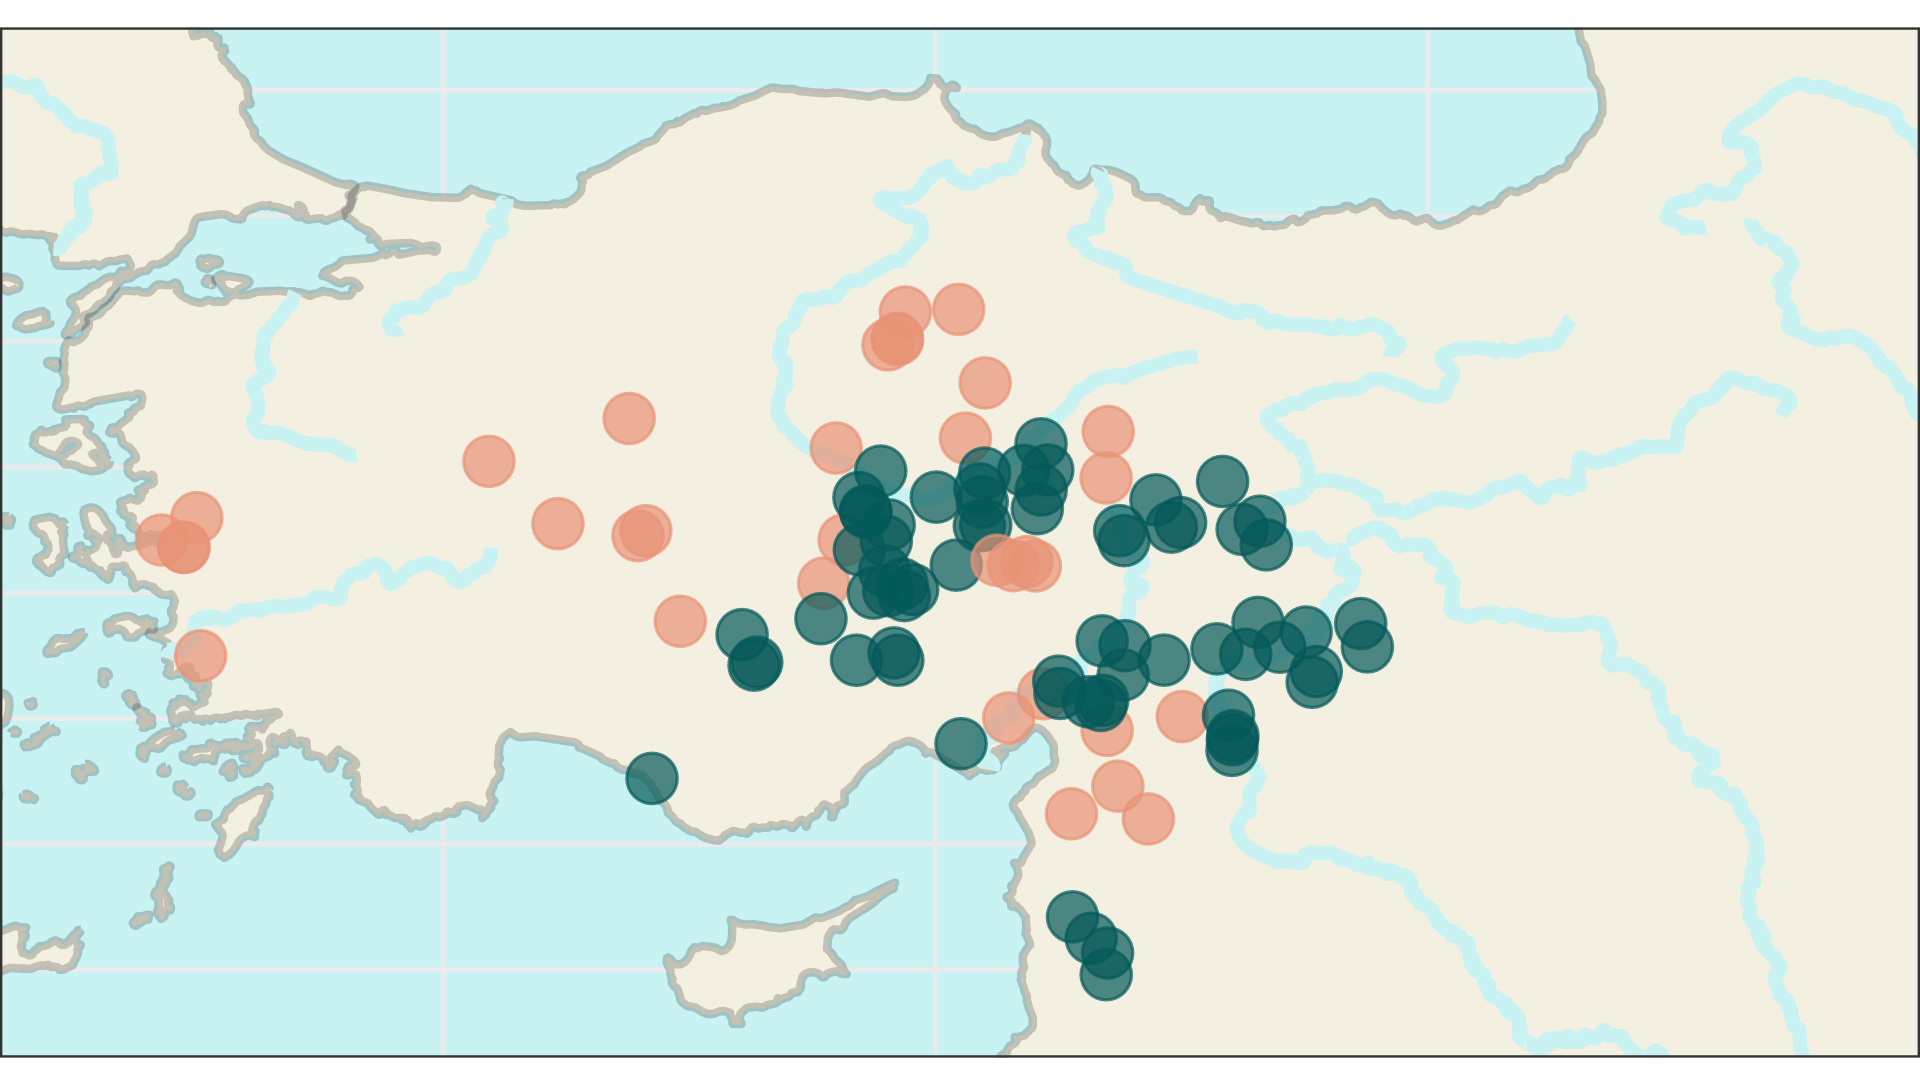
\includegraphics[width=0.95\textwidth]{../../../Mídia/MapTodo.png}
	\end{center}
	\caption{Mapa das inscrições conhecidas atualmente. Pontos laranjas
		denotam inscrições do período Imperial e pontos verdes as do período
		Neo-Hitita.
	}\label{fig:todo}
\end{figure}

\chapter{Os hieróglifos}

\begin{compactitem}
	\item Sem relação com nenhum outro sistema de escrita da região conhecido.
	\item Apenas utilizados na escrita de luvita.
	\item Direção de leitura: bustrofédon.
	\item Sistema de escrita em que cada grafema pode ter três valores:
	\begin{compactitem}
		\item Logográfico: o grafema representa um item lexical (≈ palavra),
		transliterados em latim com letras maiúsculas.
		\item Silabográfico: o grafema representa uma sílaba, em luvita apenas séries V,
		CV, CVCV.
		\item Determinativo: o grafema delimita o campo semântico da próxima
		palavra. Transliterados em latim com letras maiúsculas dentro de parênteses.
		E.g.: \luwiantrans{DEUS-ku-pa-pa-sa} (DEUS)\emph{ku-pa-pa-sa} $\rightarrow$ \emph{Kubabas} (a deusa)
	\end{compactitem}
	\item Um encontro consonantal do tipo ``C\textsubscript{1}C\textsubscript{2}V''
	é expresso por C\textsubscript{1}a-C\textsubscript{2}V, e.g:
	\luwiantrans{mu-ka-sa-sá} \emph{mu-\uline{ka-sa-}sá} $\rightarrow$
	\emph{Muksas} (o povo, talvez = frígios).
	\item Consoantes finais são grafadas como -Ca.
	\item Os logogramas podem vir acompanhados ou não de silabogramas que expressem
	parte ou a totalidade da palavra que representam, incluindo as desinências de
	caso, número, pessoa etc.
	\item Logogramas por vezes tem múltiplas leituras. Nesses casos, é comum incluir
	parte da fonologia em silabogramas.
	\item Nem sempre os silabogramas que acompanham um logograma são contíguos na
	palavra subjacente, e.g.:\ \luwiantrans{FILIUS-ni-za-sa}
	FILIUS-\emph{ni-za-sa} $\rightarrow$ \emph{ni\uline{muwi}zas} `filho' =
	\luwiantrans{FILIUS-ni-mu-wi-za-sa} FILIUS-\emph{ni-mu-wa/i-za-sa}.
\end{compactitem}


\chapter{Gramática}

\begin{compactitem}
	\item Língua flexional, desinências via de regra finais.
	\item Sistema nominal:
	\begin{compactitem}
		\item Gêneros: Comum\slash{}Animado e Neutro.
		\item Número: Singular e Plural.
		\item Casos: Nominativo, Acusativo, Genitivo, Dativo e Ablativo.
	\end{compactitem}
	\item Sistema verbal:
	\begin{compactitem}
		\item Modos finitos: Indicativo, Imperativo.
		\item Tempos: Presente e Pretérito.
		\item Número: Singular e Plural.
		\item Modos infinitos: Infinitivo, Particípio Passivo e Gerundivo.
	\end{compactitem}
	\item Ordem de palavras ``não-marcada': Sujeito-Objeto-Verbo.
	\item Cadeia de clíticos tal como no hitita.
\end{compactitem}

\chapter{Amostra de texto: HAMA }

A datação das inscrições é de aproximadamente 830 \textsc{aec}, uma vez que
o rei
Uradamis é filho de Urhilina (\emph{ass.} Irhuleni),\footnote{
	A leitura do nome de Uradamis varia dependendo do autor e
	época da publicação, sendo a mais frequente na bibliografia a forma
	Ura\textbf{ta}mis.
	Como mencionado ao longo deste curso, até~\citet{Rieken2008}, não se
	diferenciava a interpretação fonológica de
	L.100 𔑰 \emph{ta}, L.29 𔐞 \emph{tà} e L.41 𔐬\slash{}𔐫 \emph{tà}, mas hoje
	podemos com confiança realizar a correção L.41 𔐬\slash{}𔐫 \emph{tà}
	$\rightarrow$ \emph{da}. Outro problema é se há ou não uma vogal /a/ no sinal
	<ra\slash{}i>, sendo assim possível que o nome seja ou U\textbf{ra}damis ou
	U\textbf{r}damis.
	A vocalização do sinal <ra\slash{}i> é resolvida no caso de Urhilina pela
	existência da forma assíria do nome, Irhuleni.
} conhecido por sua
participação na batalha de Qarqar (853 \textsc{aec}) por meio das inscrições
do rei assírio Salmānu-ašarēd III (Salmanaser III).\footnote{Mais detalhes
	sobre Irhulani\slash{}Urhilina e Salmānu-ašarēd\slash{}Salmanaser III
	em~\citeabbrev*{RlA},
	\href{https://publikationen.badw.de/en/rla/index\#5833}{v. 05 p. 162}.
}
Ao que tudo indica, as inscrições foram encontradas na região em que foram
inicialmente produzidas e expostas, revelando a presença de cidades-estado
neo-hititas muito mais ao sul do que o antigo império hitita da era do bronze.
A inscrição está atualmente locada junto de HAMA 1 e 3 no Eski Şark Eserleri
Müzesi, Istabul (no. 7890).

\clearpage%

\begin{center}
	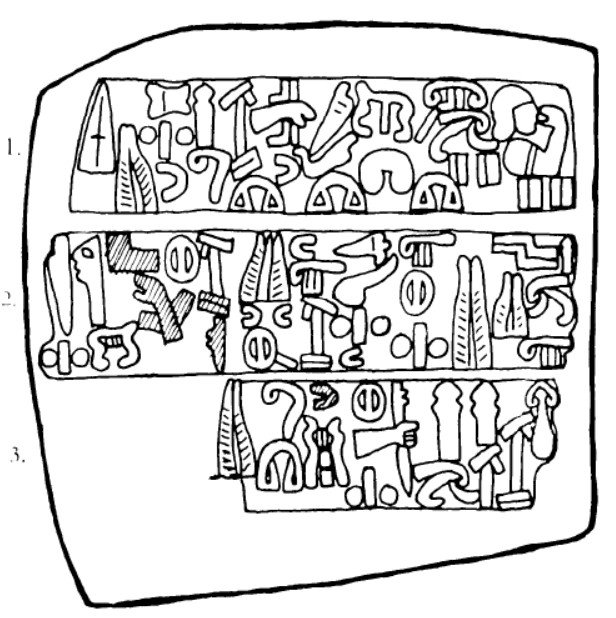
\includegraphics[width=0.85\textwidth]{../../../Mídia/hama14.jpg}
\end{center}


\begin{parnumbersa}[]
	\raggedright%

	\Large \luwiantrans{EGO-mi}\hspace{5pt}
	\luwiantrans{MAGNUS-ra-da-mi-sa}\hspace{5pt}
	\luwiantrans{u-ra-hi-li-na-sa}\hspace{5pt}
	\luwiantrans{FILIUS-ni-za-sa}\hspace{5pt}
	\luwiantrans{i-ma-tú-wa-ni REGIO}\hspace{5pt}
	\luwiantrans{REX}


	\Large \luwiantrans{a-wa}\hspace{5pt}
	\luwiantrans{á-mu}\hspace{5pt}
	\luwiantrans{AEDIFICARE-mi-ha}\hspace{5pt}
	\luwiantrans{za-a}\hspace{5pt}
	\luwiantrans{<CASTRUM>-hara-ni-sà-za}\hspace{5pt}
	\luwiantrans{la-ka-wa-ni-sà-ha-wa REGIO}\hspace{5pt}
	\luwiantrans{FLUMEN-REGIO-da-i-sà}

	\Large \luwiantrans{REL-za} \hspace{5pt}
	\luwiantrans{i-zi-i-da}\hspace{5pt}
	\luwiantrans{a-tá-ha-wa}\hspace{5pt}
	\luwiantrans{ni-ki-ma-sa REGIO}

\end{parnumbersa}

\vspace{10pt}
\hrule
\vspace{10pt}

\setcounter{parcount}{0}
\begin{parnumbersa}[]

	\raggedright%
	\itshape%

	\logo{EGO}-mi
	\logo{MAGNUS}+ra/i-da-mi-sa
	u-ra/i-hi-li-na-sa
	\logo{FILIUS}.NI-za-sa
	i-ma-tú-wa/i-ni\logo{(REGIO)} \logo{REX}

	a-wa/i á-mu \logo{AEDIFICARE}+MI-ha za-' \logo{(``CASTRUM'')}hara/i-ni-sà-za
	la-ka-wa/i-ni-sà-ha-wa/i\logo{(REGIO)} \logo{FLUMEN.REGIO}-da-i-sà

	\logo{REL}-za i-zi-i-da a-tá-ha-wa/i ni-ki-ma-sa\logo{(REGIO)}


\end{parnumbersa}

\vspace{10pt}
\hrule
\vspace{10pt}


\setcounter{parcount}{0}
\begin{parnumbersa}[]

	\raggedright%
	\itshape%
	amu=mi Uradamis Urhilinas nimuwizas imatuwani hantawatis.

	a=wa amu tamaha za harnisa=za, lakawanis hapadis

	kwa=za izida, anta=ha=wa Nikimas.


\end{parnumbersa}

\vspace{10pt}
\hrule
\vspace{20pt}


\clearpage%

\ex.[]\ag.[1] \emph{amu} \emph{=mi} \emph{Uradamis} \emph{Urhilinas}
\emph{nimuwizas} \emph{imatuwani} \emph{hantawatis.}\\
\Pro{}1\Sg{} =\Refl{}. U.-\Com{}\Nom{}\Sg{} U.-\Com{}\Gen{}\Sg{} filho-\Com{}\Nom{}\Sg{}
imatuano-\Com{}\Nom{}\Sg{} rei-\Com{}\Nom{}\Sg{}\\
Eu sou Uradamis, filho de Urhilinas, rei imatuano.
\bg.[2] \emph{a} \emph{=wa} \emph{amu} \emph{tamaha} \emph{za} \emph{harnisa=za,}\\
\Conj{} =\Clt{} \Pro{}1\Sg{} construir-1\Sg{}\Pret{} \Pro{}\Neut{}\Acu{}\Sg{}
fortaleza-\Neut{}\Acu{}\Sg{}=\Clt{}\\
E eu (mesmo) construí esta fortaleza,
\bg.[||] lakawanis =ha =wa hapadis\\
L.\Com{}\Nom{}\Sg{} =\Conj{} =\Clt{} fluvial-\Com{}\Nom{}\Sg{}\\
\bg.[3] \emph{kwa=za} \emph{izida},\\
\Rel{}\Neut{}\Acu{}\Sg{}=\Clt{} fazer-3\Sg{}\Pret{}\\
a qual o povo de Laka fez,
\bg.[] \emph{anda=ha=wa} \emph{Nikimas}.\\
dento=\Conj{}=\Clt{} N.\Com{}\Nom{}\Sg{}\\
E dentro [dela está] Nikima.


\bigskip
\begin{flushleft}
	\noindent \textbf{Tradução}\\
	\noindent [1] ``Eu sou Uradamis, filho de Urhilina, rei imatuano. [2] Eu mesmo
	construí esta fortaleza, (e foi) o povo de Laka, a região fluvial, [3] que a fez e
	dentro (da fortaleza?) está Nikima.
\end{flushleft}


\chapter*{Recomendações bibliográficas}

A maioria das inscrições, incluindo selos, grafites e cartas de Assur, estão
editadas, traduzidas e comentadas no \emph{Corpus of Hieroglyphic Luwian
	Inscriptions} organizado por Hawkins \cite{CHLI11,CHLI12,CHLI13,CHLI2,CHLI3}.
Há também uma seleta de traduções publicada por~\citet{Payne2012}.

Detalhes sobre a descoberta, publicação e decifração dos hieróglifos luvitas
podem ser encontrados em~\citet[pp. 131ff.]{HawkinsScripts}. Para uma descrição
ainda mais detalhada, ver~\citet[pp. 6-17]{CHLI11}.
O compêndio de~\citet{Melchert2003} oferece detalhes e bibliografia para todos
os aspectos da história, geografia e língua luvita.
Informações detalhadas sobre as línguas anatólicas podem ser encontradas
em~\citet[239--308]{HSK41.1} e, sobre a dialetologia do luvita,
ver~\citet{Yakubovich2010}.

O panorama geral do sistema de escrita está descrito
em~\citet[p. 155ff.]{HawkinsScripts}.
Uma discussão detalhada e atualizada sobre todos os sinais conhecidos e com
as evidências utilizadas para sua interpretação pode ser encontrada
em~\citet[354--488]{CHLI3}.
Diversos artigos sobre sinais específicos são frequentemente publicados, sendo
os mais
importantes~\citet{HawkinsMorpurgoNeumann1974,Rieken2008,RiekenYakubovich2010}.

Não há gramáticas ou dicionários de consulta compilados ainda para o luvita
hieroglífico.
O panorama gramatical está disponível no compêndio de~\citet{Melchert2003} e no
método de~\citet{Payne2010}.
A melhor fonte de consulta para o vocabulário é o último volume do \emph{Corpus
	of Hieroglyphic Luwian Inscriptions} de~\citet{CHLI13} e a bibliografia por ele
utilizada.


\printbibliography%


\end{document}
